\documentclass[article]{jss}

%% -- LaTeX packages and custom commands ---------------------------------------

%% recommended packages
\usepackage{orcidlink,thumbpdf,lmodern}

\usepackage{amssymb}
\usepackage{amsmath}
\usepackage{siunitx}

%% another package (only for this demo article)
\usepackage{framed}

%% new custom commands
\newcommand{\class}[1]{`\code{#1}'}
\newcommand{\fct}[1]{\code{#1()}}


%% -- Article metainformation (author, title, ...) -----------------------------

%% - \author{} with primary affiliation (and optionally ORCID link)
%% - \Plainauthor{} without affiliations
%% - Separate authors by \And or \AND (in \author) or by comma (in \Plainauthor).
%% - \AND starts a new line, \And does not.
\author{Fernando Ferraz Ribeiro~\orcidlink{0000-0002-0685-4774}\\Universidade Federal da Bahia
   \And Gilney Figueira Zebende~\orcidlink{0000-0003-2420-9805}\\Universidade Estadual\\de Feira de Santana}
\Plainauthor{Fernando Ferraz Ribeiro, Gilney Figueira Zebende}
%  and $DMC_x^2$
%% - \title{} in title case
%% - \Plaintitle{} without LaTeX markup (if any)
%% - \Shorttitle{} with LaTeX markup (if any), used as running title
\title{A \proglang{Python}/\proglang{Zig} optimized and customizable implementation for the $\rho_{DCCA}$ and $DMC_x^2$ methods}
\Plaintitle{A Python/Zig optimized and customizable implementation for the Pdcca and DMCx2 methods}
\Shorttitle{\proglang{Python}/\proglang{Zig} implementation for the $\rho_{DCCA}$ and $DMC_x^2$}

%% - \Abstract{} almost as usual
\Abstract{
  This paper presents tha \pkg{Zebende}, a \proglang{Python} package written in \proglang{Python} and \proglang{Zig}, that calculates the $DFA$, $DCCA$ $\rho_{DCCA}$ and the $DMC_x^2$. The package presents an optimized algorithm that significantly improves the calculations speed. A comparison with other packages that calculates the .The package is also the first to implement the $DMC_x^2$ coefficient for any number of series.
}

%% - \Keywords{} with LaTeX markup, at least one required
%% - \Plainkeywords{} without LaTeX markup (if necessary)
%% - Should be comma-separated and in sentence case.
\Keywords{$\rho_{DCCA}$, $DMC_x^2$, optimization, \proglang{Python}, \proglang{Zig}}
\Plainkeywords{Pdcca, DMCx2, optimization, Python, Zig}

%% - \Address{} of at least one author
%% - May contain multiple affiliations for each author
%%   (in extra lines, separated by \emph{and}\\).
%% - May contain multiple authors for the same affiliation
%%   (in the same first line, separated by comma).
\Address{
  Fernando Ferraz Ribeiro\\
  Universidade Federal da Bahia\\
  Faculty of Achitecture\\
  Universit\"at Innsbruck\\
  Universit\"atsstr.~15\\
  6020 Innsbruck, Austria\\
  E-mail: \email{fernando.ribeiro@ufba.br}\\
  \emph{and}\\
  Centro Universitário Senai-Cimatec\\

  % URL: \url{https://www.zeileis.org/}
}

\begin{document}


%% -- Introduction -------------------------------------------------------------

%% - In principle "as usual".
%% - But should typically have some discussion of both _software_ and _methods_.
%% - Use \proglang{}, \pkg{}, and \code{} markup throughout the manuscript.
%% - If such markup is in (sub)section titles, a plain text version has to be
%%   added as well.
%% - All software mentioned should be properly \cite-d.
%% - All abbreviations should be introduced.
%% - Unless the expansions of abbreviations are proper names (like "Journal
%%   of Statistical Software" above) they should be in sentence case (like
%%   "generalized linear models" below).

\section{introduction} \label{sec:intro}

The Detrended Cross-correlation Coefficient ($\rho_{DCCA}$)~\citep{Zebende2011} is a widely used coefficient that measures the cross-correlation between tow non-stationary time series. It´s an extension of the Detrended Fluctuation Analysis ($DFA$)~\citep{Peng_1994} and the Detrended Cross-correlation Analysis ($DCCA$)~\citep{Podobnik2008}: while the $DFA$ calculates the self-affinity and long-memory properties of a time series data, and the $DCCA$ analyses power-law cross correlations between two different non-stationarity time series, the $\rho_{DCCA}$ coefficient quantifies this cross-correlation in simple values ranging from $-1$ to $1$, where $-1$ indicates a perfect anti-correlation between the series, $1$ a perfect correlation and zero ($0$) no correlation at all.

% rho DCCA applications

The Detrended Multiple Cross-Correlation Coefficient \citep{Zebende2018} ($DMC_x^2$) is a generalization of the $\rho_{DCCA}$ coefficient that correlates one time series (dependent variable) a number of time series (independent variables). The $DMC_x^2$ values ranges from zero ($0$), indicating no correlation to $1$, meaning perfect correlation or anti-correlation between the dependent and the independent variables.

% DMCx2 applications

This paper presents the \pkg{Zebende} \proglang{Python} package, an implementation of the $DFA$, $DCCA$, $\rho_{DCCCA}$, $DMC_x^2$ and utility functions related to the methods. In section \ref{sec:calculations} the steps for calculating the $\rho_{DCCCA}$ and $DMC_x^2$ are presented and discussed. Section \ref{sec:optimization} shows how this library was implemented, the optimization technics and the recommended steps to use the library. In Section \ref{sec:results} the \pkg{Zebende} package is compared with other packages for \proglang{Python} and \proglang{R} that calculates the $\rho_{DCCA}$ in terms of performance and usability, leading to the conclusions in Section \ref{sec:summary}.

\section{Algorithms of the coefficients}\label{sec:calculations}

The algorithms that calculates the $\rho_{DCCA}$ uses the $DFA$ and the $DCCA$ steps. The $DMC_x^2$ coefficient uses the $\rho_{DCCA}$ coefficient and, consequently, also embraces the $DFA$ and the $DCCA$. The $DFA$ method is described in six steps:


\begin{enumerate}\label{steps:dfa}

  \item Taking a time series $\{x_{i}\}$ with $i$ ranging from $1$ to $N$, the integrated series $X_{k}$ is calculated by $X_{k} = \sum_{i=1}^{k}\left[x_{i} - \langle x \rangle \right]$ with \(k\) also ranging from $1$ to $N$;
  \item the  $X_{k}$ series is divided in $N - n$ boxes of size $n$(time scale), each box containing $n + 1$ values, starting in $i$ up to $i + n$;
  \item for each box, a polynomial (usually of degree 1) best fit is calculated, getting $\widetilde{X}_{k, i}$ with $i \le k \le (i + n)$;
  \item in each box is calculated: $f_{DFA}^{2}(n, i) = \frac{1}{1+n} \sum_{k=i}^{i + n}(X_{k}-\widetilde{X}_{k})^{2}$
  \item for all the boxes of a time scale, the $DFA$ is calculated as:\\[10pt]
        $F_{DFA}(n) = \sqrt{\frac{1}{N - n} \sum_{i=1}^{N-n} f_{DFA}^{2}(n, i)}$;
  \item for a number of different timescales ($n$), with possible values $4 \le n \le \frac{N}{4}$ the $F_{DFA}$ function is calculated to find a relation among $F_{DFA} \times n$

\end{enumerate}


The $DCCA$ method is very similar to the $DFA$ calculations, with the difference of analyzing two series while the $DFA$ evaluate properties of a single time series. It´s also a six steps process:


\begin{enumerate}
  \label{steps:DCCA}
  \item Taking two time series with the same length $\{x\alpha_{i}\}$ and $\{x\beta_{i}\}$ with $i$ ranging from $1$ to $N$,
        the integrated series $X\alpha_{k}$ and $X\beta_{k}$ are calculated by
        $X_{k} = \sum_{i=1}^{k}\left[x_{i} - \langle x \rangle \right] $ for each series, with $k$ also ranging from $i$ to $N$;
  \item $X\alpha_{k}$ and $X\beta_{k}$ series are divided in $N - n$ boxes of size $n$(time scale), each box containing $n + 1$ values, starting in $i$ up to $i + n$;
  \item for each box, a polynomial (usually of degree 1) best fit is calculated, getting
        $\widetilde{X\alpha}_{k, i}$ and $\widetilde{X\beta}_{k, i}$,
        for series $\{x\alpha_{i}\}$ and $\{x\beta_{i}\}$ respectively,
        with $i \le k \le (i + n)$;
  \item in each box is calculated: $f_{DCCA}^{2}(n, i) =
          \frac{1}{1+n} \sum_{k=i}^{i + n}(X\alpha_{k}-\widetilde{X\alpha}_{k, i}) \times (X\beta_{k}-\widetilde{X\beta}_{k})$
  \item for all the boxes of a time scale, the $DCCA$ is calculated as:\\[10pt]
        $F_{DCCA}^{2}(n) =\frac{1}{N - n} \sum_{i=1}^{N-n} f_{DCCA}^{2}(n, i)$;
  \item for a number of different timescales ($n$), with possible values
        $4 \le n \le \frac{N}{4}$ the $F_{DCCA}^{2}$ function is calculated to find a relation among
        $F_{DCCA}^{2} \times n$
\end{enumerate}

Comparing the algorithms, the first three are basically identical, the only difference is that the $DCCA$ method apply those steps to two series. The step four of the $DFA$ can be considered an analogous of the variance, replacing the average subtraction (in the variance) for the values obtained by the polinomial fit(estimated seires); and the equivalent step of the $DCCA$ is, in the same terms, compared to the covariance between the two series. The technique of fitting a curve, interpreted as a trend inside each box, and subtracting the value estimated by the trend from the actual value in the integrated series $(X_{k}-\widetilde{X}_{k})$ from now on will be called \textbf{detrended values}($DV$). In the $DFA$ algorithm, the $f_{DFA}^{2}(n, i)$ function is the mean of the square of the $DV$, in $DCCA$ calculations, the $f_{DCCA}^{2}(n, i)$ function evaluates the mean of the product of the $DV$ of the two series in each box.

Step five of the $DFA$ calculates the square root of the mean of the values calculates in the previous step for each box, in the $DCCA$, the mean of the values evaluated for each box is calculated in stead. The last step, in both cases, is more a reminder to repeat the respective previous operations for a number of difference time scales ($n$).

The $\rho_{DCCA}$ is measured using Eq. \ref{eq:p_dcca}. Considering the relation between $DFA$ and variance and $DCCA$ and covariance, the $\rho_{DCCA}$ resembles Pearson correlation for a time scale $n$.

\begin{equation}
  {\rho}_{DCCA}(n) = \frac{F_{DCCA~(x\alpha,~x\beta)}^{2}(n)}
  {F_{DFA~(x\alpha)}(n) \times F_{DFA~(x\beta)}(n)}
  \label{eq:p_dcca}
\end{equation}

The $DMC_x^2$ is a generalization of the $\rho_{DCCA}$ that calculates the correlation between one time-series $\left\lbrace Y \right\rbrace $, as the  dependent variable, and a number $j$ of time-series $\left\lbrace X_{1} \right\rbrace $, $\left\lbrace X_{2} \right\rbrace $, $\left\lbrace X_{3} \right\rbrace $, $\dots $, $\left\lbrace X_{j} \right\rbrace $ defined as independent variables. The coefficient is expressed mathematically as:

\begin{equation}
  {DMC}_{x}^{2}  \equiv \rho_{Y,X_{i}}(n)^{T} \times \rho^{-1}(n) \times \rho_{Y,X_{i}}(n)
  \label{eq:dmcx2}
\end{equation}

In Eq. \ref{eq:dmcx2}, $\rho^{-1}(n)$ represent the inverse of a matrix populated by all possible combinations of $\rho_{DCCA}$ between independent variables. In Eq. \ref{eq:p_dcca_matrix}, value $\rho_{X_{1},X_{2}}(n)$, for instance, is the $\rho_{DCCA}$ for independent variables $X_{1}$ and $X_{2}$ calculated with time scale $n$, occupying position $\rho_{1 2}$ of the matrix. Two fundamental characteristics: the first is that the main diagonal values are all ones, since it's position in the matrix denotes the calculation of a cross-correlation between a series and itself. Second, the matrix is symmetric in relation to the main diagonal, as the $\rho_{DCCA}$ is a commutative operation.

\begin{equation}
  \rho^{-1}(n) = \left(\begin{matrix}
    1                     & \rho_{X_{1},X_{2}}(n) & \rho_{X_{1},X_{3}}(n) & \dots & \rho_{X_{1},X_{j}}(n) \\
    \rho_{X_{2},X_{1}}(n) & 1                     & \rho_{X_{2},X_{3}}(n) & \dots & \rho_{X_{2},X_{j}}(n) \\
    \vdots                & \vdots                & \vdots                & \dots & \vdots                \\
    \rho_{X_{j},X_{1}}(n) & \rho_{X_{j},X_{2}}(n) & \rho_{X_{j},X_{3}}(n) & \dots & 1                     \\
  \end{matrix}\right)^{-1}
  \label{eq:p_dcca_matrix}
\end{equation}

At last Eq. \ref{eq:rhocol} represent the transposed vector of the $\rho_{Y,X_{i}}(n)$ between the depended variable $\left\lbrace Y \right\rbrace $ and each $\left\lbrace X_{i} \right\rbrace $ independent variable for a given time scale $n$.

\begin{equation} \label{eq:rhocol}
  \rho_{Y,X_i}(n)^T=[\rho_{Y,X_1}(n), \rho_{Y,X_2}(n),\cdots,\rho_{Y,X_j}(n)]
\end{equation}

As the $DFA$ and the $DCCA$,~$\rho_{DCCA}$ and~$DMC_x^2$ should be evaluated in a number of time scales ($n$) to analyze the characteristics of each coefficient.

%% -- Manuscript ---------------------------------------------------------------

%% - In principle "as usual" again.
%% - When using equations (e.g., {equation}, {eqnarray}, {align}, etc.
%%   avoid empty lines before and after the equation (which would signal a new
%%   paragraph.
%% - When describing longer chunks of code that are _not_ meant for execution
%%   (e.g., a function synopsis or list of arguments), the environment {Code}
%%   is recommended. Alternatively, a plain {verbatim} can also be used.
%%   (For executed code see the next section.)

\section{Zebende package: implementation and optimization} \label{sec:optimization}

The implementation of the \pkg{Zebende} package follows some well defined golas:

\begin{enumerate}
  \item Enhance performance;
  \item avoid redundant calculations;
  \item make the outputs compatibles with other data analyses tools (including data manipulation, machine learn and statistical packages);
  \item create a customizable and modular set of tools;
  \item facilitate package evolution and maintenance;
  \item deliver an easy to use package.
\end{enumerate}

The \proglang{Python} language was chosen because it´s one of the most used languages in the data analyses field and have a great support for statistical tools and machine learning algorithms. The are a pletora of tools to load and manipulate data (\pkg{Pandas}, \pkg{Polar}, \pkg{PySpark} ...), execute statistical analyzes (\pkg{Numpy}, \pkg{SciPy}, \pkg{StatsModels} ...), machine learning (\pkg{Pytorch}, \pkg{TensorFlow}, \pkg{Scykit Learn}...) and data visualization(\pkg(Matplotlib), \pkg{Seaborn}, \pkg{Plotly} ...) among other related applications.

\begin{figure}[h!]
  \centering
  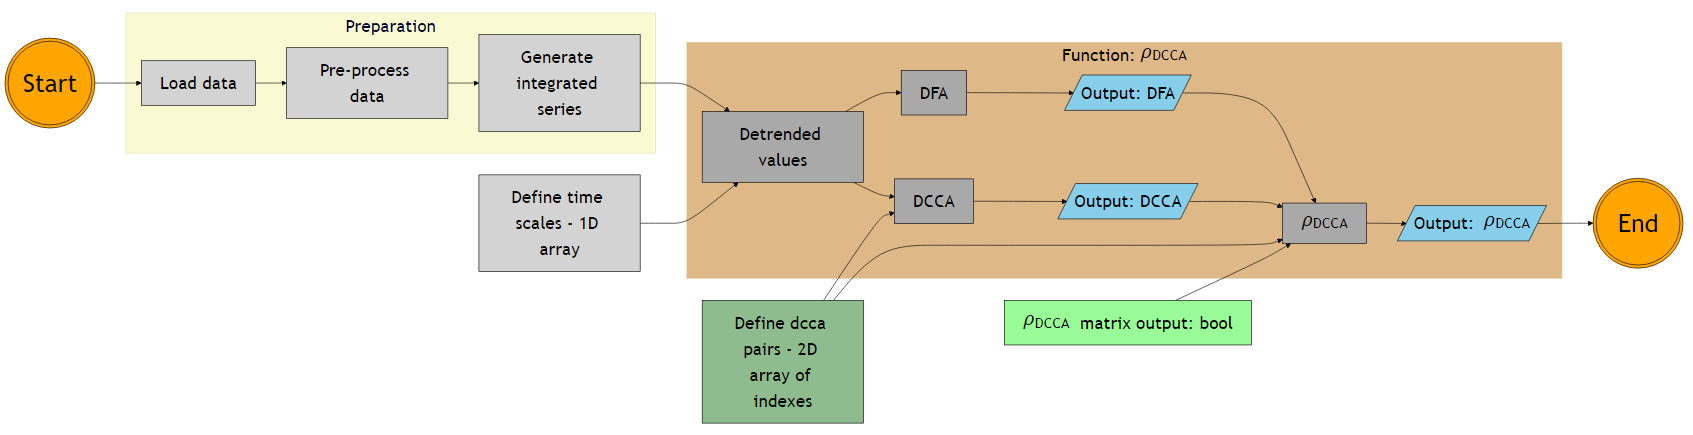
\includegraphics{./figs/pdcca_chart.png}
  \caption{\label{fig:pdcca_chart}Calculating  $\rho_{DCCA}$ with \pkg{Zebende} package - Simplified flowchart}
\end{figure}

The first draft of the code was written in pure \proglang{Python}, to rapidly prototype the way users will interact with the package. Figures \ref{fig:pdcca_chart} and \ref{fig:dmc_chart} presents simplified flowcharts illustrating how to use the package and how the main functions ($\rho_{DCCA}$ and $DMA_x^2$) works.

\begin{figure}[h!]
  \centering
  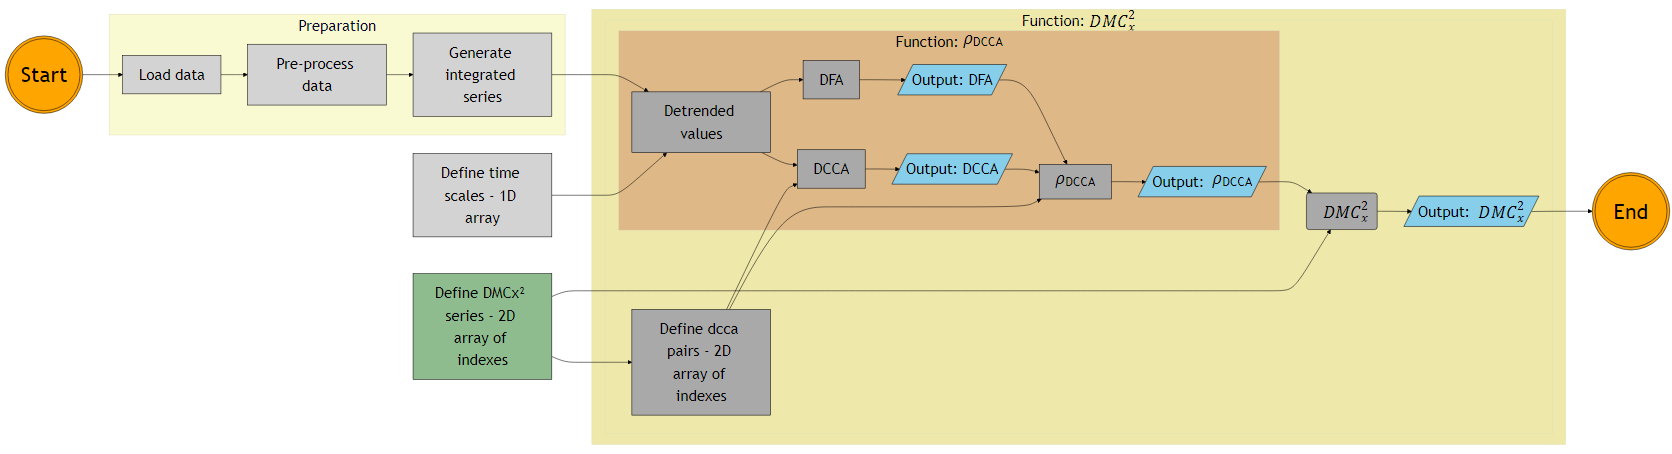
\includegraphics{./figs/dmc_chart.png}
  \caption{\label{fig:dmc_chart}Calculating  $DMC_x^2$ with \pkg{Zebende} package - Simplified flowchart}
\end{figure}

The preparation steps are the same in both functions. First the data is loaded, and should be analyzed by the researchers. Base on the data characteristics, the set should be treated to ensure the methods requirements in the "Pre-processing" stage. The package functions expects data as ma matrix with the columns as the series and the lines as time steps. Columns unused in the indented research should also be dropped for better performance os the algorithms in this step. The more common way to do that is to use a data manipulation package. To proceed to the next step, the data table should be in the form of a \pkg{Numpy} 2D array, and this could be done with any data manipulation \proglang{Python} package. The next step is to calculate the integrated series. The package provides a function, named \verb"integrated_series()", to calculate that. The code example below show how to load the libraries (using \pkg{Pandas} as the data manipulation packages and loading a \verb".csv" file as a generic example), convert to \pkg{Numpy} array and generate the integrated series.

\begin{Code}
# importing packages
import numpy as np
import pandas as pd
import zebende as zb

data = pd.read_csv('path_to_the_file.csv') # loading data
# Pre-processing data
# ...
data = data.to_numpy(data) #converting data to Numpy array
int_data = zb.integrated_series(data) # calculating the integrated series
\end{Code}

The option of taking out the integrated series generation from the main functions to an independent one was inspired by \cite{Peng_1994} work, where the way of calculating integrated series was different from the one that is widely used in more recent years. The integration of the series is essentially a pre-processing step, and this approach makes easy to explore alternative ways to integrate the series or compare \cite{Peng_1994} approach to the current one in different scenarios.

The input and output structures of each function are displayed below:

\begin{Code}
def p_dcca(
    input_data: NDArray[float64],
    tws: NDArray[int64] | NDArray[float64],
    DCCA_of: ndarray | Literal['all'] = "all",
    P_DCCA_output_matrix: bool = False
) -> tuple[NDArray[float64],  # DFA
          NDArray[float64],   # DCCA
          NDArray[float64]    # P_DCCA
          ]
\end{Code}

\begin{Code}
def dmcx2(
    input_data: NDArray[float64],
    tws: NDArray[int64] | NDArray[float64],
    dmcx2_of: ENUM_DMCx2_of | NDArray[float64] | list = 'all-full'
) -> tuple[ NDArray[float64],   # DFA
            NDArray[float64],   # DCCA
            NDArray[float64],   # P_DCCA
            NDArray[float64],   # DMC
          ]
  \end{Code}

The first two inputs are the same for functions \verb"p_dcca()" and \verb"dmcx2()": \verb"input_data" receive the integrated series and the \verb"tws" receives an 1D array representing the time scales (box size) described in the algorithms on Section \ref{sec:calculations}. The \verb"input_data" is a 2D array of 64 bits floating point data. The \verb"tws" accepts integers and, for convenience reasons, also floating points. Since the size of the boxes needs to be integers, in case of floating points, the values will be converted to integers by ignoring the decimal values(truncating). This two inputs are colored in light gray in Figures \ref{fig:pdcca_chart} and \ref{eq:dmcx2}, indicating mandatory inputs.

With the mandatory steps explained, some very important optional inputs should be addressed. Starting with the $\rho_{DCCA}$ function (dark green node in Figure \ref{fig:dmc_chart}) represents the input \verb"DCCA_of" of the function. This input requires a 2D array of integers, each row is a pair of index, related to the \verb"data_input" matrix. For example: if the \verb"input_data" receives a four columns matrix, with index ranging from $0$ to $3$, that is intended to calculate de $DFA$ for all the series but the $\rho_{DCCA}$ between series of index $0$ and $1$ and also for series $2$ and $3$, the \verb"DCCA_of" input should receive the array \verb"[[0,1], [2,3]]". If no value (or the string \verb"'all'") is given, the function will calculate all possible combinations of $DCCA$ calculations between all the series respecting the index values order, as below:

\begin{Code}
[[0,1], [0,2], [0,3], [1,2], [1,3], [2,3]]
\end{Code}

It´s important to understand the calculation steps, the role of the \verb"DCCA_of" array and how it fits in the goals of the package implementation. The code below is part of the \proglang{Python} implementation of the $\rho_{DCCA}$ function, 

\begin{Code}
for n_index, n  in enumerate(tws): # for each time scale
  # temporaty allocation arrays
  f2dfa_n = np.full(shape=(data.shape[0] - n, data.shape[1]),
  fill_value=np.nan, dtype=data.dtype)
  dcca_n = np.full(shape=(data.shape[0] - n, DCCA_of.shape[0]), 
  fill_value=np.nan, dtype=data.dtype)
  detrended_mat = np.full(shape=(n + 1, data.shape[1]), 
  fill_value=np.nan, dtype=data.dtype)
  for i in range(data.shape[0] - n): # for each box
      detrended_series( # inputs
                        time_steps[i : i + (n + 1)],  # arr_x
                        data[i : i + (n + 1), :],  # mat_y
                         detrended_mat,  # output
                      )
      f2dfa_n[i] = np.power(detrended_mat, 2).mean(axis=0)
      for j, pair in enumerate(DCCA_of): # for each DCCA pair
          dcca_n[i, j] = (detrended_mat[:, pair[0]] * detrended_mat[:, pair[1]]
                         ).mean(axis=0)
  F_DFA_arr[n_index, :] = np.sqrt(f2dfa_n.mean(axis=0))
  DCCA_arr[n_index, :] = dcca_n.mean(axis=0)
  # calculation of P_DCCA
  P_DCCA_output_function(n_index, DCCA_of, F_DFA_arr, DCCA_arr, # Inputs
  P_DCCA_arr) # Output
\end{Code}

The first \verb"for" loop in the code operates over the values of the \verb"tws" input, asserting that the step 6 of the $DFA$ and $DCCA$ methods in Section \ref{sec:calculations}. Three temporary arrays are allocated for each time scale. The first, \verb"f2dfa_n", to store the calculations of the step 4 of the $DFA$. The number of lines of this array correspond to the number of boxes in the current time scale ($N - n$) and the columns is the number of series in the analysis. Array  \verb"dcca_n", holds the values calculated in the step 4 of the $DCCA$. The number of lines also correspond to the number of boxes but the number of columns equals the number of pairs (rows) in the \verb"DCCA_of" input. The \verb"detrended_mat" array has a number of lines is the number of points in a time scale box ($n +1$) and column count also equal to the number of time series. This last array is very important to the implementation goals.

In each box, the \verb"detrended_series" function execute a one degree polynomial fit, subtract the values of the serie with the value given by the interpolated curve and stores this values in the \verb"detrended_mat". After the $DFA$ is calculated. With all the detrended values calculated, another loop, for all the rows in the \verb"DCCA_of", uses the \verb"detrended_mat" and the $DFA$ arrays to calculate the $DCCA$. This approach avoid redundant calculation. If the \verb"DCCA_of" is $[[0,1], [0,2], [1,2]]$, the detrended and $DFA$ values for each serie are calculated just once. If in a set of four series, a research intend to calculate the $DCCA$ between the first serie and all the others along with the two last series, inputting  \verb"DCCA_of" $= [[0,1], [0,2], [0,3], [2,3]]$. In this case, the \verb"detrended_mat" will be calculated just once for each series and the $DCCA$ between series $[[1,2], [1,3]]$ will be skipped, revealing a very customizable algorithm. 

The function named \verb"P_DCCA_output_function" in the code above,is a pointer to other functions. One that outputs the  $\rho_{DCCA}$ results in the form of a table (rows for each time scale and columns for each \verb"DCCA_of" pair) and the other outputs it the form of a 3D matrix, where each level is the matrix in Equation \ref{eq:p_dcca_matrix} for one of the time scales. This behavior is driven by the \verb"P_DCCA_output_matrix" input (represented as the light green node in Figure \ref{fig:pdcca_chart}), where \verb"False" means table output and \verb"True" matrix output. This is very convenient for calculating the $DMC_x^2$. There are two utility functions to transform a table output in a matrix one (\verb"p_dcca_simple_to_matrix") and also the other way around (\verb"p_dcca_matrix_to_simple").

The \verb"dmcx2" function runs the \verb"p_dcca()" with \verb"P_DCCA_output_matrix" set to \verb"True". There is no \verb"DCCA_of" input for the $DMC_x^2$ function, instead there is a \verb"dmcx2_of" parameter. This input receives a 2D matrix where each line represents the indexes of the series to be used in Equation \ref{eq:dmcx2}. The first value of each row is the index of the serie used as the dependent variable, the others, the independent ones. There are two literal strings that can be used, for convenience as inputs for this parameter: \verb"'all-full'", that generates a 2D array with every series as the dependent variable against all the others; and \verb"'first-full'", with only one row, having the index zero series as the dependente variable in relation with all the others. The \verb"'all-full'" option is operated by the function \verb"dmc_of_all_as_y".

There is a restriction to the \verb"dmcx2_of" array: the independent values must be in crescent order. There is a check in the \verb"dmcx2" that raises an error if the values are out of order, and suggests the use of a utility function named \verb"ordering_x_dmcx2_of". The code below shows an example of a manually defined \verb"dmcx2_of" array with 2 elements out of order in the second row, the \verb"AssertionError" output, the way of fixing it with the \verb"ordering_x_dmcx2_of" function and finally the outputted ordered array.

\begin{CodeChunk}
  \begin{CodeInput}
dmcx2_of = np.array([ [0, 1, 2, 3],
                      [1, 0, 3, 2],
                      [2, 0, 1, 3],
                      [3, 0, 1, 2]  ])

dfa , dcca, pdcca, dmc = zb.dmcx2(int_data, tws, dmcx2_of=dmcx2_of)
  \end{CodeInput}
  \begin{CodeOutput}
AssertionError: 
dmcx2_of x values out of order: 
use zebende.ordering_x_dmcx2_of(dmcx2_of)
 to fix it before passing the dmcx2_of values to zebende.dmcx2() function"
  \end{CodeOutput}
  \begin{CodeInput}
dmcx2_of = ordering_x_dmcx2_of(dmcx2_of)
print(dmcx2_of)
  \end{CodeInput}
  \begin{CodeOutput}
[[0 1 2 3]
 [1 0 2 3]
 [2 0 1 3]
 [3 0 1 2]]
  \end{CodeOutput}
\end{CodeChunk}





%% -- Illustrations ------------------------------------------------------------

%% - Virtually all JSS manuscripts list source code along with the generated
%%   output. The style files provide dedicated environments for this.
%% - In R, the environments {Sinput} and {Soutput} - as produced by Sweave() or
%%   or knitr using the render_sweave() hook - are used (without the need to
%%   load Sweave.sty).
%% - Equivalently, {CodeInput} and {CodeOutput} can be used.
%% - The code input should use "the usual" command prompt in the respective
%%   software system.
%% - For R code, the prompt "R> " should be used with "+  " as the
%%   continuation prompt.
%% - Comments within the code chunks should be avoided - these should be made
%%   within the regular LaTeX text.

\section{Results} \label{sec:results}




%% -- Summary/conclusions/discussion -------------------------------------------

\section{Summary and discussion} \label{sec:summary}


%% -- Optional special unnumbered sections -------------------------------------

% \section*{Computational details}

% \begin{leftbar}
%   If necessary or useful, information about certain computational details
%   such as version numbers, operating systems, or compilers could be included
%   in an unnumbered section. Also, auxiliary packages (say, for visualizations,
%   maps, tables, \dots) that are not cited in the main text can be credited here.
% \end{leftbar}

% The results in this paper were obtained using
% \proglang{R}~3.4.1 with the
% \pkg{MASS}~7.3.47 package. \proglang{R} itself
% and all packages used are available from the Comprehensive
% \proglang{R} Archive Network (CRAN) at
% \url{https://CRAN.R-project.org/}.


% \section*{Acknowledgments}

% \begin{leftbar}
%   All acknowledgments (note the AE spelling) should be collected in this
%   unnumbered section before the references. It may contain the usual information
%   about funding and feedback from colleagues/reviewers/etc. Furthermore,
%   information such as relative contributions of the authors may be added here
%   (if any).
% \end{leftbar}


%% -- Bibliography -------------------------------------------------------------
%% - References need to be provided in a .bib BibTeX database.
%% - All references should be made with \cite, \citet, \citep, \citealp etc.
%%   (and never hard-coded). See the FAQ for details.
%% - JSS-specific markup (\proglang, \pkg, \code) should be used in the .bib.
%% - Titles in the .bib should be in title case.
%% - DOIs should be included where available.

\bibliography{refs}


%% -- Appendix (if any) --------------------------------------------------------
%% - After the bibliography with page break.
%% - With proper section titles and _not_ just "Appendix".

% \newpage

% \begin{appendix}

%   \section{More technical details} \label{app:technical}

%   \begin{leftbar}
%     Appendices can be included after the bibliography (with a page break). Each
%     section within the appendix should have a proper section title (rather than
%     just \emph{Appendix}).

%     For more technical style details, please check out JSS's style FAQ at
%     \url{https://www.jstatsoft.org/pages/view/style#frequently-asked-questions}
%     which includes the following topics:
%     \begin{itemize}
%       \item Title vs.\ sentence case.
%       \item Graphics formatting.
%       \item Naming conventions.
%       \item Turning JSS manuscripts into \proglang{R} package vignettes.
%       \item Trouble shooting.
%       \item Many other potentially helpful details\dots
%     \end{itemize}
%   \end{leftbar}


%   \section[Using BibTeX]{Using \textsc{Bib}{\TeX}} \label{app:bibtex}

%   \begin{leftbar}
%     References need to be provided in a \textsc{Bib}{\TeX} file (\code{.bib}). All
%     references should be made with \verb|\cite|, \verb|\citet|, \verb|\citep|,
%     \verb|\citealp| etc.\ (and never hard-coded). This commands yield different
%     formats of author-year citations and allow to include additional details (e.g.,
%     pages, chapters, \dots) in brackets. In case you are not familiar with these
%     commands see the JSS style FAQ for details.

%     Cleaning up \textsc{Bib}{\TeX} files is a somewhat tedious task -- especially
%     when acquiring the entries automatically from mixed online sources. However,
%     it is important that informations are complete and presented in a consistent
%     style to avoid confusions. JSS requires the following format.
%     \begin{itemize}
%       \item JSS-specific markup (\verb|\proglang|, \verb|\pkg|, \verb|\code|) should
%             be used in the references.
%       \item Titles should be in title case.
%       \item Journal titles should not be abbreviated and in title case.
%       \item DOIs should be included where available.
%       \item Software should be properly cited as well. For \proglang{R} packages
%             \code{citation("pkgname")} typically provides a good starting point.
%     \end{itemize}
%   \end{leftbar}

% \end{appendix}

%% -----------------------------------------------------------------------------


\end{document}
